\documentclass{beamer}
%\documentclass[handout]{beamer}
\usepackage{etex}
\usepackage[utf8]{inputenc}
\usepackage[T1]{fontenc}
\usepackage[ngerman]{babel}
\usepackage{color}
\usepackage{colortbl}
\usepackage{amsmath}
\usepackage{amsfonts}
\usepackage{amssymb}
\usepackage{mathabx}
\usepackage{textcomp}
\usepackage{natbib}
\usepackage{multirow}
\usepackage{nicefrac}
\usepackage{multicol}
\usepackage{url}
\usepackage{gb4e-}
\usepackage{pifont}

\title[Topic Domains]{Automatic Classification by Topic Domain for Meta Data Generation, Web Corpus Evaluation, and Corpus Comparison}
\author[Roland Schäfer, Felix Bildhauer]{Roland Schäfer$^1$ and Felix Bildhauer$^2$}
\institute[]{$^1$German Grammar, Freie Universität Berlin (DFG, grant SCHA1916\slash 1-1)\\ $^2$Institut für Deutsche Sprache, Mannheim}
\date[]{10th Web as Corpus Workshop (WAC-X), ACL 2016, Berlin\\August 12, 2016}

\usetheme{default}
\usecolortheme{beaver}

\newcommand*\rot{\rotatebox{90}}

\begin{document}

%\titlegraphic{\includegraphics[width=0.2\textwidth]{fulogo}\hspace{0.05\textwidth}
\includegraphics[width=0.125\textwidth]{dfglogo}\hspace{0.25\textwidth}
\includegraphics[width=0.2\textwidth]{idslogo}}
%\frame{\titlepage}

\begin{frame}
%\begin{textblock*}%{2cm}(.35cm,-8cm)                                                                                          
%  \includegraphics[scale=.48]{hukombi_bwb}
\includegraphics[width=0.25\textwidth]{graphics/fulogo}\hspace{0.05\textwidth}
\includegraphics[width=0.10\textwidth]{graphics/dfglogo}\hspace{0.3\textwidth}
\includegraphics[width=0.25\textwidth]{graphics/idslogo}
%  \end{textblock*}
  \maketitle
\end{frame}


\begin{frame}
  {Background}
  \begin{itemize}
    \item \alert{Reliable metadata}: not available for large crawled web corpora
    \item \alert{Topic domain} (and genre/register) meta data:\\
      essential to many corpus linguists
    \item Also important for \alert{corpus evaluation} and corpus comparison\\
%      \citep{Kilgarriff2001,BiemannEa2013,SchaeferBildhauer2013de}
      \vspace{0.5cm}
\pause
    \item Automatic classification by \alert{genre/register}: in unrestricted domains, disappointing results, even in recent experiments
    \item \citet{BiberEgbert2016}: acc.=0.42, prec.=0.27, rec.=0.3
  \end{itemize}
\end{frame}


\begin{frame}
  {Automatic classification by content}  
  \begin{itemize}
    \item Promising results years ago already \citep{Sebastiani2002}
    \item \alert{Data-driven induction of topics}: a very objective way\\
      of organizing a collection of documents by content
    \item Topic classification through internal criteria:\\ also advocated in the \citet{EAGLES1996} guidelines
   \end{itemize}
  
  \vspace{0.5cm}     
\pause
  But:
  \begin{itemize}
    \item \alert{Topic modeling}: no category labels
    \item From a linguist's viewpoint: categories should be\\
      `intuitively' interpretable
  \end{itemize}
  \end{frame}


  \begin{frame}
    {Experiment}
    Idea
    \begin{enumerate}
      \item Infer a topic distribution over a corpus using\\
	topic modeling algorithms (\alert{unsupervised})
      \item Do not interpret the inferred topical structure directly
      \item Instead, learn a small set of topic domains from\\
	the documents' assignment to the topics (\alert{supervised})
    \end{enumerate}
\pause
    Goals
    \begin{itemize}
      \item Development of a suitable annotation scheme\\
	for topic domain, grounded in lexical distributions
      \item Corpus comparison: web corpus vs.\ newspaper corpus\\
       (very little is known about the composition\\
       of crawled web corpora)
    \end{itemize}
    \end{frame}


\begin{frame}
  {CoReCo}
%  Text classification schema  \citep{SchaeferBildhauer2012a}\\
%
%  \begin{itemize}
%    \item No complex categories such as \textit{genre}, \textit{register} etc.
%    \item Instead simple categories: \textit{Aim}, \textit{Mode}, \alert{\textit{Topic Domain}}
%    \item Builds on previous work by \citet{Sharoff2006}
%    \end{itemize}
%\pause
    Custom classification schema for topic domains\\
    \footnotesize{\url{http://corporafromtheweb.org/cowcat/}}

    \begin{itemize}
    \item Design goal: moderate number (about 10--20) of topic domains\\
    (broad subject areas)
    \item Basis for our classifcation experiment reported here: 13 categories
    \item Developed in a cyclic fashion\\
    (repeated annotation processes, annotator feedback)
  \end{itemize}
\end{frame}

\begin{frame}
  {Step 1: Creating a gold standard data set}
  \begin{itemize}
    \item 870 documents from \alert{DECOW14}, crawled \alert{web} corpus\\
    \citep{SchaeferBildhauer2012a,Schaefer2015b}
    \item 886 documents from \alert{DeReKo}, mostly \alert{newspaper} texts\\
    \citep{KupietzEa2010}
    \item Manually annotated with CoReCo categories\\
      \vspace{0.5cm}
    {\footnotesize Annotators: Sarah Dietzfelbinger, Lea Helmers, Theresia Lehner,\\
    Kim Maser, Samuel Reichert, Luise Rißmann (FU Berlin);\\
  Monica Fürbacher (IDS Mannheim)}
  \end{itemize}
\end{frame}


\begin{frame}
  {Distribution of topic domains}
  Comparison of DeReKo and DECOW14\\[1cm]
  \begin{center}
    
\includegraphics[width=0.45\textwidth]{graphics/dereko-cowcat}~
\includegraphics[width=0.45\textwidth]{graphics/cow-cowcat}
  \end{center}
\end{frame}

\begin{frame}
  {Step 2: Topic modeling}

  \begin{itemize}
    \item Starting point: term-document matrix
    \item Topics: defined by a set of weighted terms
    \item Documents: weighted assignment to topics
  \end{itemize}
  \vspace{.5cm}
\pause
  Our experiment:
  \begin{itemize}
    \item LSI (\citealp{LandauerDumais1994})\\
          LDA (\citealp{BleiEa2003})\\
          as implemented in \texttt{Gensim} \citep{RehurekSojka2010}% \nocite{LandauerDumais1994,LandauerDumais1997,BleiEa2003})
    \item LDA topic distributions unstable (small gold standard corpora)
    \item Results reported here are from LSI topic modelling
 %   \item Incrementally add other documents from the source copora
 %    \vspace{.25cm}
%\pause
%    \item Input terms: lemma $+$ simplified POS tag (\textit{kindergarten\_nn}) 
%    \item Filtering: best results with lower-cased, purely alphabetic noun lemmas, 4--30 chars long
    \end{itemize}
\end{frame}


\begin{frame}
  {Corpus comparison: distribution of (selected) LSI-topics}
  \begin{center}
    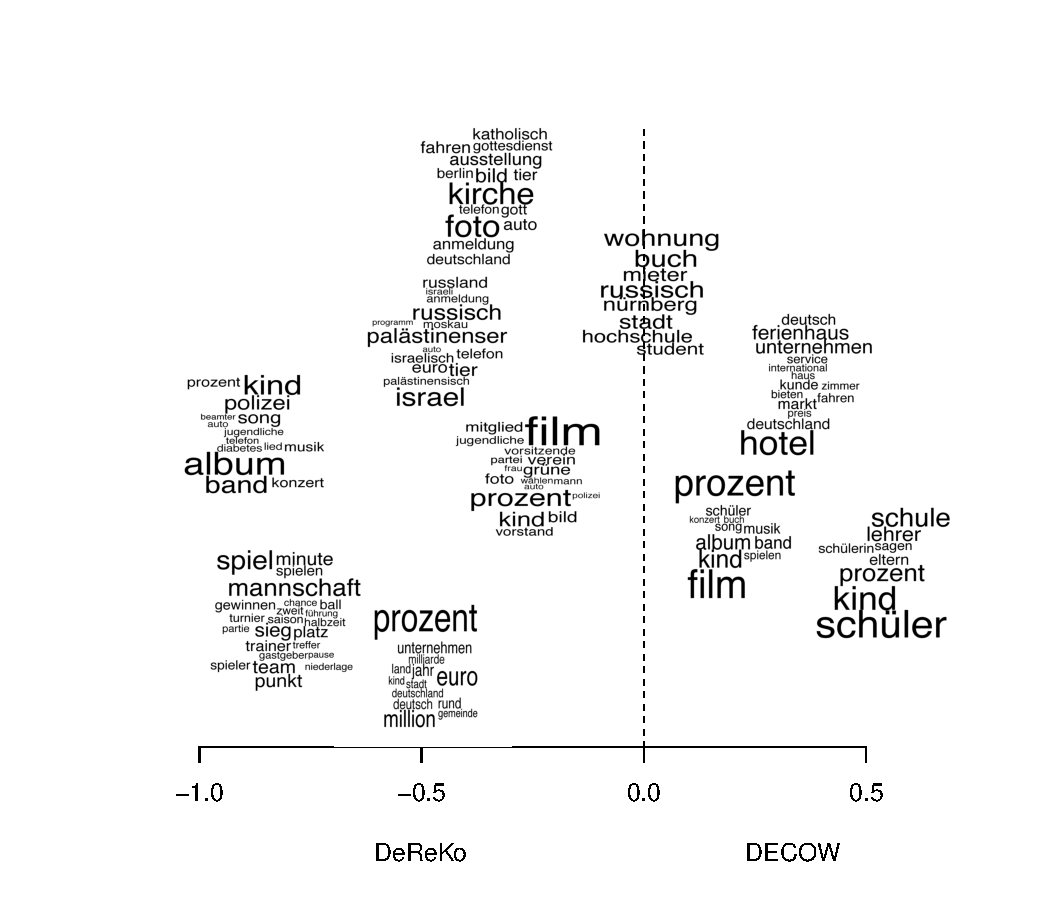
\includegraphics[width=0.75\textwidth]{graphics/topics-logratios2bw}
  \end{center}
\end{frame}




\begin{frame}
  {Step 3: Learning CoReCo topic domains from LSI-topics}
  \begin{itemize}
    \item Permutation of virtually all supervised classifiers in \texttt{Weka}\\ \citep{HallWitten2011}
    \item Highest accuracy: SVMs with a Pearson VII universal kernel\\ \citep{UstunEa2006}
  \end{itemize}
  \vspace{.5cm}
\pause
Set of experiments with:
  \begin{itemize}
    \item varying number of LSI-topics
    \item topics induced from
      \begin{itemize} 
        \item gold standard data plus varying amounts\\
	  of additional documents
        \item several pre-processing variants
      \end{itemize}
    \item evaluation on the \textit{full} data set and on a \textit{reduced} data set (with rare categories removed)
  \end{itemize}
\end{frame}


\begin{frame}
  {Results: Web (accuracy)}
%Best result: $acc=68.765\%$,  $prec=0.688$, $rec=0.688$, $F=0.674$\\
  \begin{figure}
    \centering
    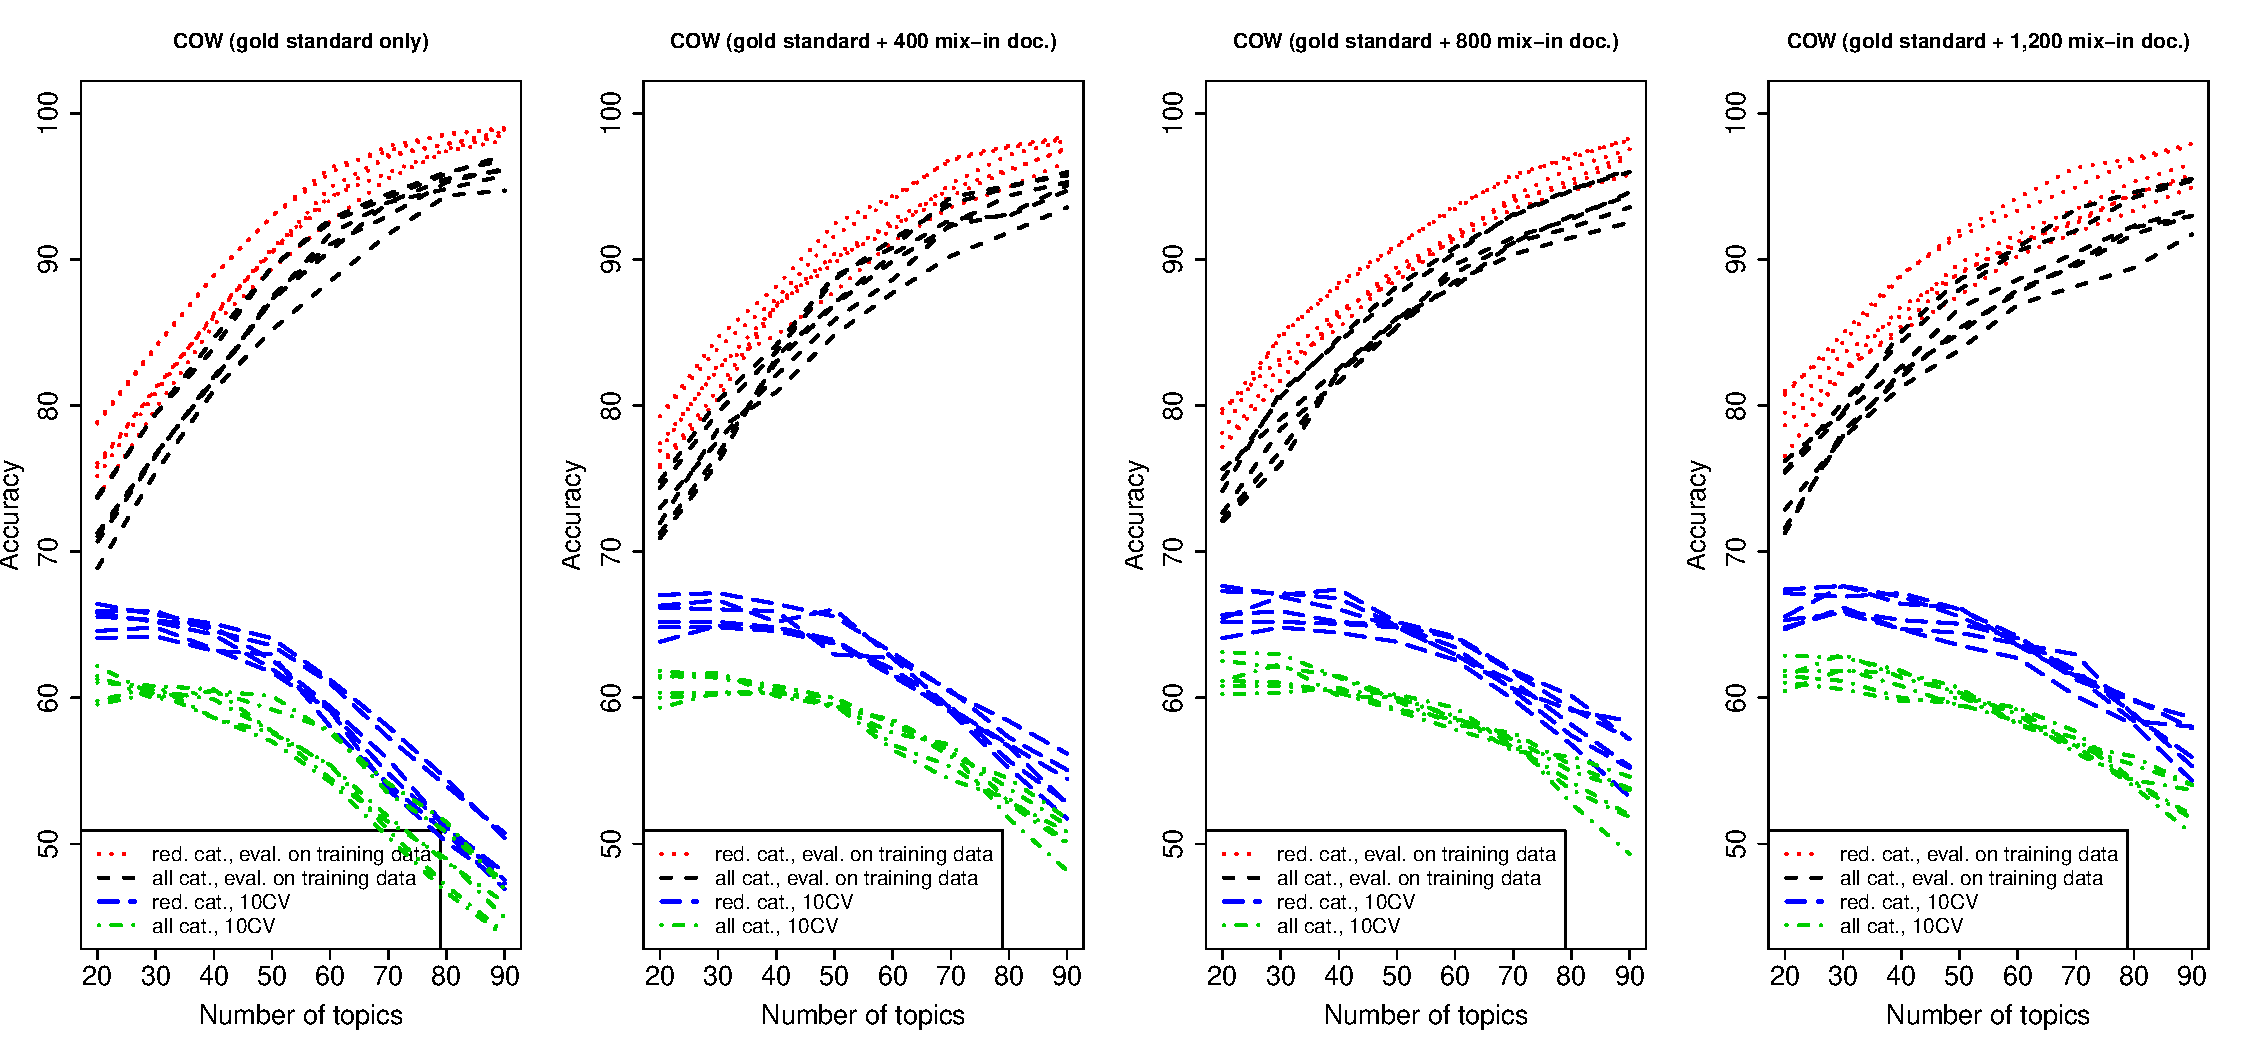
\includegraphics[width=\textwidth, height=6.4cm]{graphics/acc_cow.pdf}
  \end{figure}
  \vspace{-.3cm}
  \centering
  \scalebox{.7}{
  \begin{tabular}{|rlrrrrr|}
      \hline
      \textbf{Mixed-in} & \textbf{Attribute} & \textbf{Topics} & \textbf{Accuracy} & \textbf{Precision} & \textbf{Recall} & \textbf{F-Measure}\\
      \hline
      3,200 & token & 20 & 68.765\% & 0.688 & 0.688 & 0.674 \\
      \hline
  \end{tabular}
  }
\end{frame}


\begin{frame}
  {Results: News (accuracy)}
  %$acc=72.999\%$, $prec=0.725$, $rec=0.730$, $F=0.696$ \\
  \begin{figure}
    \centering
    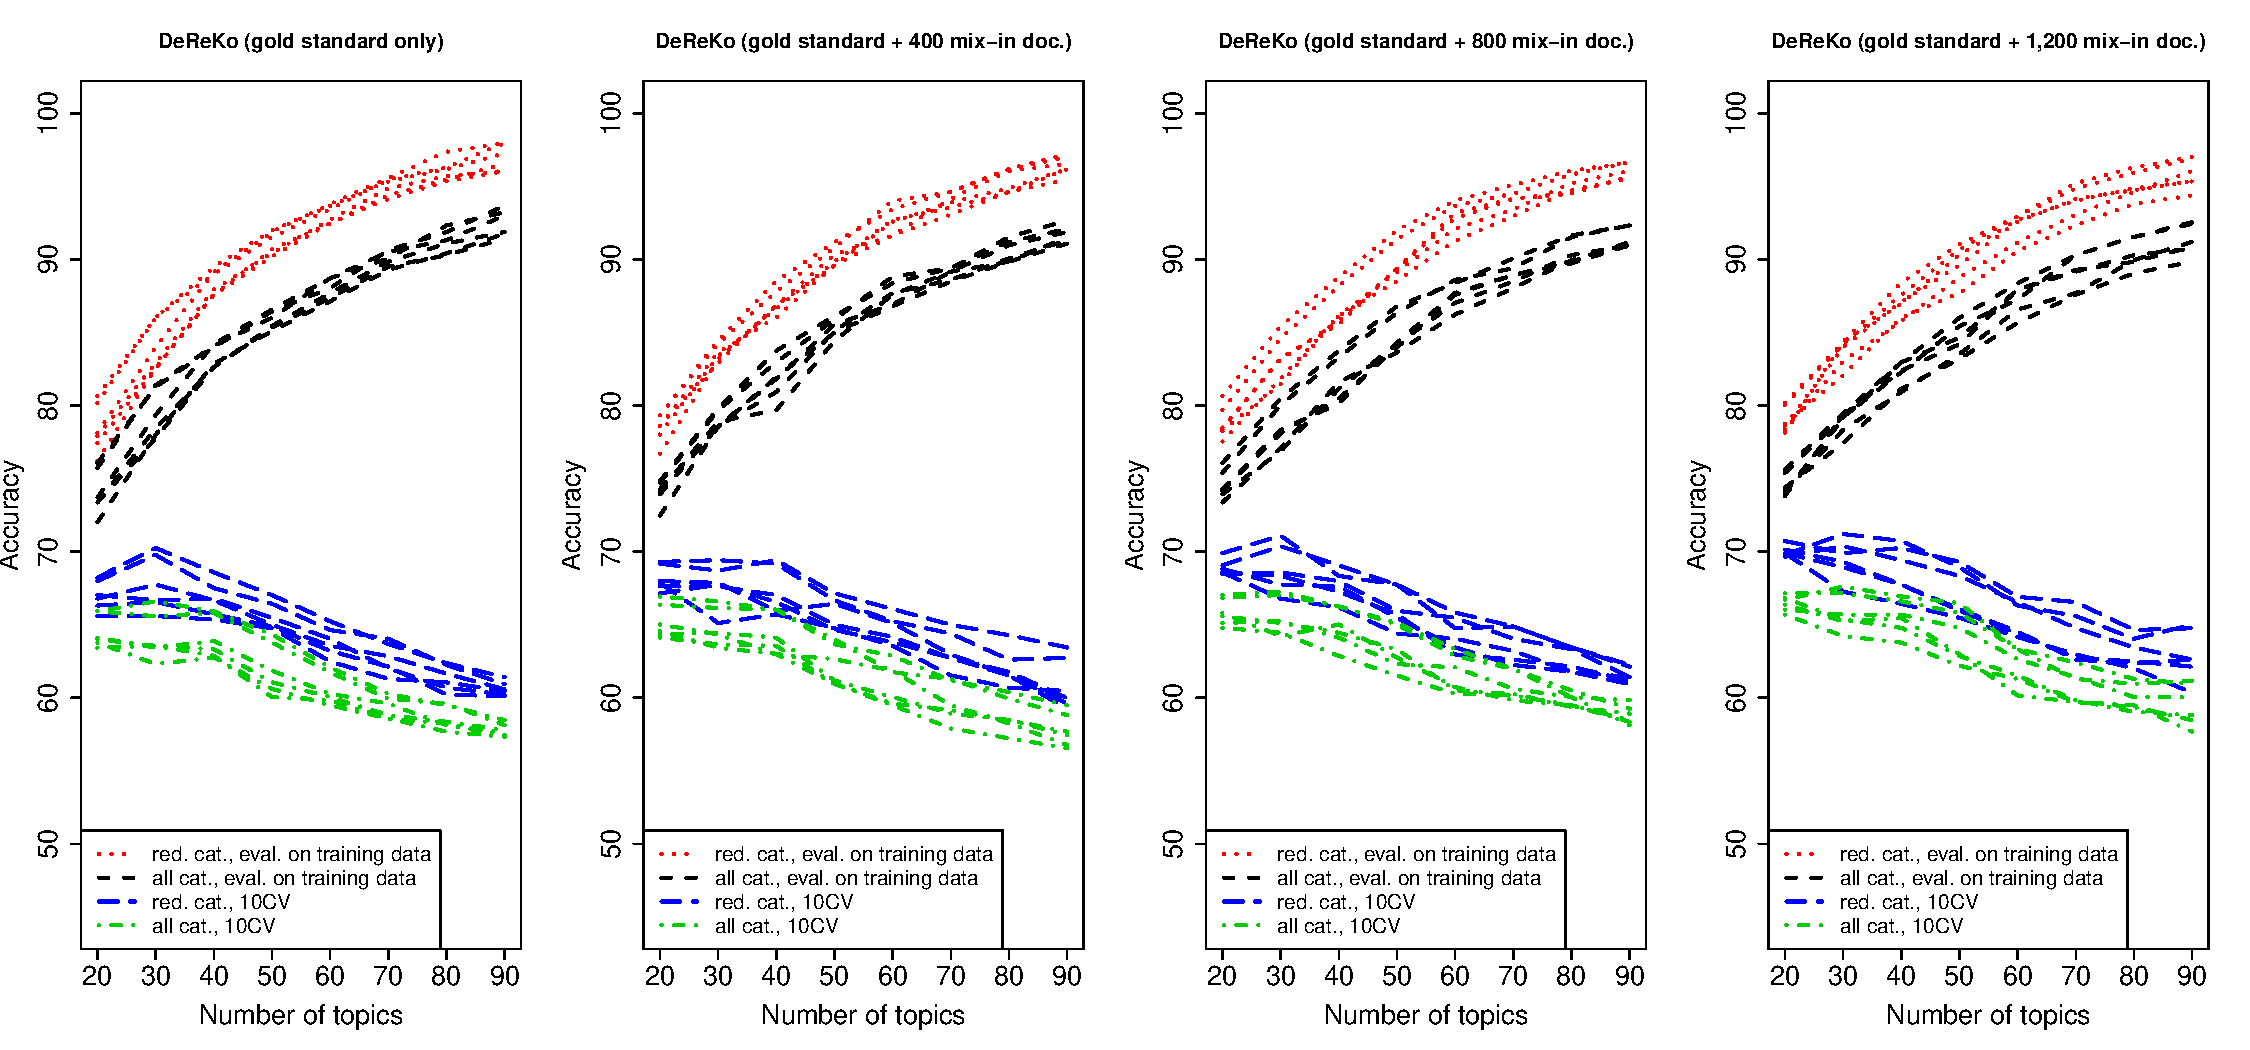
\includegraphics[width=\textwidth, height=6.4cm]{graphics/acc_dereko.pdf}
  \end{figure}
  \vspace{-.3cm}
  \centering
  \scalebox{.7}{
    \begin{tabular}{|rlrrrrr|}
      \hline
      \textbf{Mixed-in} & \textbf{Attribute} & \textbf{Topics} & \textbf{Accuracy} & \textbf{Precision} & \textbf{Recall} & \textbf{F-Measure}\\
      \hline
      3,600 & lemma + POS & 40 & 72.999\% & 0.725 & 0.730 & 0.696 \\     
      \hline
    \end{tabular}
  }
\end{frame}

\begin{frame}
  {Results: Web + News (accuracy)}
\pause
  %$acc=72.999\%$, $prec=0.725$, $rec=0.730$, $F=0.696$ \\
  \begin{figure}
    \centering
    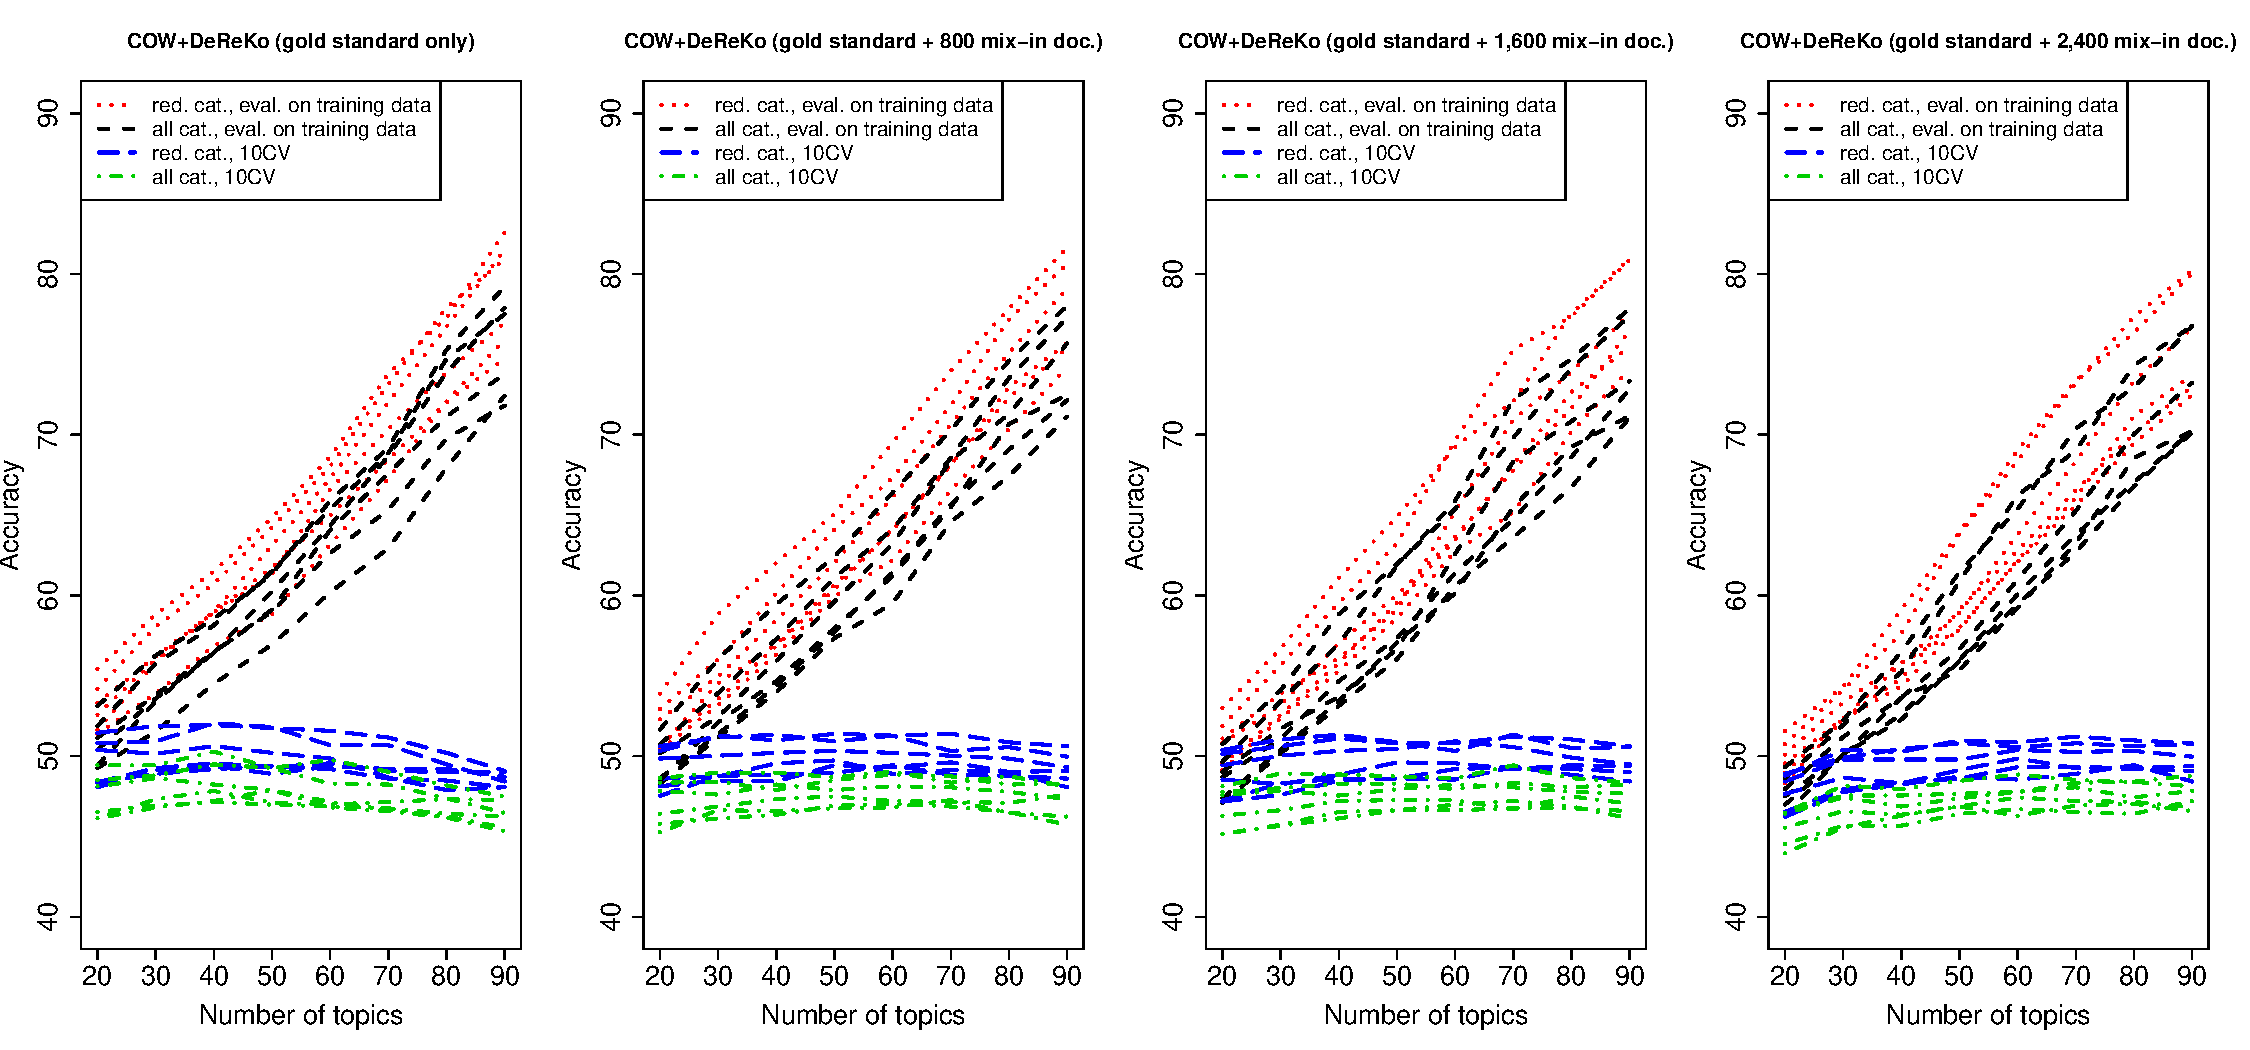
\includegraphics[width=\textwidth, height=6.4cm]{graphics/acc_coreko.pdf}
  \end{figure}
  \vspace{-.3cm}
  \centering
  \scalebox{.7}{
    \begin{tabular}{|rlrrrrr|}
      \hline
      \textbf{Mixed-in} & \textbf{Attribute} & \textbf{Topics} & \textbf{Accuracy} & \textbf{Precision} & \textbf{Recall} & \textbf{F-Measure}\\
      \hline
      0 & lemma + POS & 30 & 51.872\% & 0.431 & 0.519 & 0.417 \\      
      \hline
    \end{tabular}
  }
\end{frame}



\begin{frame}
  {Results: all}
  \centering
  \scalebox{.65}{
    \begin{tabular}{|lrllrrrr|}
      \hline
      \textbf{Corpus} & \textbf{Mixed-in} & \textbf{Attribute} & \textbf{Topics} & \textbf{Accuracy} & \textbf{Precision} & \textbf{Recall} & \textbf{F-Measure}\\
      \hline
      Web & 3,200 & token & 20 & 68.765\% & 0.688 & 0.688 & 0.674 \\
      News & 3,600 & lemma + POS & 40 & 72.999\% & 0.725 & 0.730 & 0.696 \\
      Web + News & 0 & lemma + POS & 30 & 51.872\% & 0.431 & 0.519 & 0.417 \\ 
      \hline
    \end{tabular}
  }

\vspace{.5cm}

  \begin{itemize}
    \item \alert{Web + News}: larger training set does not increase accuracy
    \item \alert{Web + News}: mixing in more documents for topic modeling does not increase accuracy
    \item \alert{News} data are even more skewed than web data\\ (two modal categories: \textit{Politics-and-Society}, \textit{Life-and-Leisure})
      \begin{itemize}
        \item higher accuracy (4.23\%) with \alert{News} data probably a side effect of the more skewed distribution
        \item \alert{Web + News}: classifier assigns most texts to \textit{Life and Leisure},\\ and the remaining texts mostly to \textit{Politics and Society}
      \end{itemize}
  \end{itemize}
\end{frame}

\begin{frame}
  {Conclusions}
  \begin{itemize}
    \item Connection between induced topic distributions\\
      and more general topic domains
\pause
    \vspace{.25cm}
    \item Decreased performance on joint Web and News corpora:
    \begin{itemize}
      \item use larger gold standard training set
      \item train separate models for Web and News data
    \end{itemize}
\pause
    \vspace{.25cm}
    \item Adapt annotation scheme
    \begin{itemize}
      \item split up some topic domains (based on annotator feedback)
      \item current experiments: multiple weighted assignments\\
	of documents to topic domains
    \end{itemize}
\pause
    \vspace{.25cm}
    \item Ultimate goal: automatically annotate existing web corpora with meta data release the data freely
  \end{itemize}
\pause
\pause
\pause
\end{frame}


\begin{frame}
  {Appendix: confusion matrices}
  \vspace{0.5cm}
  \resizebox{0.5\textwidth}{!}{\begin{tabular}{|llcccccccc|}
    \hline
    \multicolumn{2}{|c}{\textbf{COW}} & \multicolumn{8}{c|}{\textbf{Classified}} \\
     && \rot{\textbf{PolSoc~}} & \rot{\textbf{Busi}} & \rot{\textbf{Life}} & \rot{\textbf{Arts}} & \rot{\textbf{Public~}} & \rot{\textbf{Law}} & \rot{\textbf{Beliefs~}} & \rot{\textbf{Hist}} \\
   \hline
   \multirow{8}{*}{\rot{\textbf{Annotated}}} & \textbf{PolSoc}  & \alert{26} &  12 &  10 &   1 &   1 &   0 &   1 &   0 \\ 
     & \textbf{Busi}    &  5 & \alert{105} &  40 &   7 &   1 &   2 &   1 &   1 \\ 
     & \textbf{Life}    &  3 &  14 & \alert{286} &   6 &   4 &   1 &   1 &   1 \\ 
     & \textbf{Arts}    &  3 &   2 &  36 &  \alert{78} &   1 &   0 &   2 &   6 \\ 
     & \textbf{Public}  &  0 &   3 &  11 &   0 &   \alert{9} &   1 &   0 &   0 \\ 
     & \textbf{Law}     &  3 &   9 &   8 &   0 &   1 &   \alert{8} &   0 &   0 \\ 
     & \textbf{Beliefs} &  4 &   3 &  11 &   6 &   1 &   0 &  \alert{30} &   1 \\ 
     & \textbf{Hist}    &  9 &   0 &   9 &   7 &   1 &   1 &   2 &  \alert{15} \\ 
     \hline
 \end{tabular}}~~\resizebox{0.4\textwidth}{!}{\begin{tabular}{|llcccccc|}
    \hline
     \multicolumn{2}{|c}{\textbf{DeReKo}} & \multicolumn{6}{c|}{\textbf{Classified}} \\
     && \rot{\textbf{PolSoc~}} & \rot{\textbf{Busi}} & \rot{\textbf{Life}} & \rot{\textbf{Indiv}} & \rot{\textbf{Arts}} & \rot{\textbf{Public}} \\
    \hline
     \multirow{6}{*}{\rot{\textbf{Annotated}}}& \textbf{PolSoc}  & \alert{223} & 6 & 39 &  0 &  0 &  8 \\
     & \textbf{Busi}    &  20 & \alert{24} &   9 &  0 &  0 &  0 \\
     & \textbf{Life}    &  24 &  1 & \alert{324} &  0 &  0 &  1 \\
     & \textbf{Indiv}   &   5 &  0 &  17 &  \alert{0} &  0 &  1 \\
     & \textbf{Arts}    &   2 &  0 &  28 &  0 &  \alert{6} &  0 \\
     & \textbf{Public}  &  35 &  0 &  30 &  0 &  0 & \alert{34} \\
    \hline
 \end{tabular}}

  \vspace{.3cm}

\resizebox{0.5\textwidth}{!}{\begin{tabular}{|llccccccccc|}
    \hline
     \multicolumn{2}{|c}{\textbf{Joint}} & \multicolumn{9}{c|}{\textbf{Classified}} \\
     && \rot{\textbf{PolSoc~}} & \rot{\textbf{Busi}} & \rot{\textbf{Medical~}} & \rot{\textbf{Life}} & \rot{\textbf{Arts}} & \rot{\textbf{Public~}} & \rot{\textbf{Law}} & \rot{\textbf{Beliefs~}} & \rot{\textbf{Hist}} \\
    \hline
    \multirow{9}{*}{\rot{\textbf{Annotated}}} & \textbf{PolSoc}   & \alert{199} &   7 &   0 & 109 &   0 &  12 &   0 &   0 &   0 \\ 
    & \textbf{Busi}     &  18 &  \alert{23} &   0 & 172 &   0 &   2 &   0 &   0 &   0 \\ 
    & \textbf{Medical}  &   6 &   0 &   \alert{0} &  29 &   0 &   1 &   0 &   0 &   0 \\ 
    & \textbf{Life}     &  25 &   4 &   0 & \alert{632} &   0 &   5 &   0 &   0 &   0 \\ 
    & \textbf{Arts}     &   2 &   2 &   0 & 160 &   \alert{0} &   0 &   0 &   0 &   0 \\ 
    & \textbf{Public}   &  46 &   2 &   0 &  56 &   0 &  \alert{19} &   0 &   0 &   0 \\ 
    & \textbf{Law}      &   8 &   0 &   0 &  31 &   0 &   0 &   \alert{0} &   0 &   0 \\ 
    & \textbf{Beliefs}  &   0 &   0 &   0 &  59 &   0 &   0 &   0 &   \alert{0} &   0 \\ 
    & \textbf{Hist}     &   4 &   0 &   0 &  50 &   0 &   0 &   0 &   0 &   \alert{0} \\ 
    \hline
 \end{tabular}}

\end{frame}

%\begin{frame}
%  {Aktuell}
%  Was die Ergebnisse nahelegen\dots\\
%
%  \vspace{0.5cm}
%
%  \begin{itemize}
%    \item größere Goldstandards
%    \item Aufteilen überstark repräsentierter Kategorien
%    \item im Projekt \textit{linguistische Webcharakterisierung} (FU Berlin):\\
%      5000 Goldstandard-Dokumente angestrebt
%      \vspace{0.5cm}
%
%    \item<2-> Aber: \alert{Brauchen wir wirklich interpretierbare Kategorien?}
%  \end{itemize}
%\end{frame}

% --------------- REFS + APPENDIX

\begin{frame}[allowframebreaks]
  {References}
  \def\newblock{\hskip .11em plus .33em minus .07em}
  \footnotesize
%  \bibliographystyle{abbrvnat} 
  \bibliographystyle{natbib.fullname}
  \bibliography{coreko}
\end{frame}

\end{document}
